%%%%%%%%%%%%%%%%%%%%%%%%%%%%%%%%%%%%%%%%%%%%%%%
%%%This is a science homework template. Modify the preamble to suit your needs. 
%The junk text is   there for you to immediately see how the headers/footers look at first 
%typesetting.


\documentclass[11pt]{article}

%AMS-TeX packages
\usepackage{amssymb,amsmath,amsthm}
%geometry (sets margin) and other useful packages
\usepackage{alltt}
\usepackage{booktabs}
\usepackage{enumerate}
\usepackage{fullpage}
\usepackage{graphicx,ctable,booktabs}
\usepackage{hyperref}
\newcommand{\ignore}[1]{}
\newcommand{\pr}{\mathbb{P}}
%
%Redefining sections as problems
%
\makeatletter
\newenvironment{problem}{\@startsection
       {section}
       {1}
       {-.2em}
       {-3.5ex plus -1ex minus -.2ex}
       {2.3ex plus .2ex}
       {\pagebreak[3]%forces pagebreak when space is small; use \eject for better results
       \large\bf\noindent{Problem }
       }
       }
       {%\vspace{1ex}\begin{center} \rule{0.3\linewidth}{.3pt}\end{center}}
       \begin{center}\large\bf \ldots\ldots\ldots\end{center}}
\makeatother



\DeclareMathOperator*{\sd}{sd}


%
%
%Contents of problem set
%    
\begin{document}

\begin{center}
  \large
  \textbf{Homework \#1 -- Due Thursday, Jul.~12, before class} \\
  STAT-UB.0001 -- Statistics for Business Control \\
\end{center}
\thispagestyle{empty}

\noindent   Some of the homework assignments will involve data files.  All data
files will be available on NYU Classes under the ``Datasets'' section.  You are
permitted to work in teams, but each student must independently write up their
own solutions (no direct copying).

Electronic submissions are not accepted, but you can write your solutions on a laptop and print it out. Print out and turn in your Minitab plots. See the ``Minitab Tips'' on NYU Classes  for tips on opening files and printing or saving plots.

\begin{problem}{}
Much of our understanding of prehistoric peoples comes from caves, such as cave paintings, evidence of fire pits, etc.  made nearly 40,000 years ago. Based on these, people tend to believe that most of prehistoric peoples lived in caves for most of their lives. Do you see any problem in this?

\vspace{0.2cm}
\textit{Solution:} Prehistoric people are associated with caves because that is where the data still exists, not necessarily because most of them lived in caves for most of their lives.  If there had been paintings on trees, animal skins or hillsides, they would have been washed away long ago. Similarly, evidence of fire pits, middens, burial sites, etc. are most likely to remain intact to the modern era in caves. 
\end{problem}{}



\begin{problem}{}
Consider these values:
\[
  21 \hspace{1em}
  22 \hspace{1em}
  18 \hspace{1em}
  25 \hspace{1em}
  27 \hspace{1em}
  9 \hspace{1em}
  21 \hspace{1em}
  34 \hspace{1em}
  20 \hspace{1em}
  16 
\]
Find the mean, median, mode, and standard deviation for these. You need to compute these values by hand. This is for you to get familiar with those formulas.

\vspace{0.2cm}
\textit{Solution:} The mean is 21.3. Sort the numbers from low to high:
$$\{9, 16, 18, 20, 21, 21, 22, 25, 27, 34\}$$
The median is the average of 5-th and 6-th number, thus 21. The mode is 21 (occurs twice). 
The sample variance is 
\begin{align*}
    s^2 &=\frac{1}{10-1}\Big[  (9-21.3)^2+(16-21.3)^2+(18-21.3)^2\\
     & +(20-21.3)^2+(21-21.3)^2+(21-21.3)^2\\
     & +(22-21.3)^2+(25-21.3)^2+(27-21.3)^2+(34-21.3)^2 \Big]\\
     &= 44.46
\end{align*}
The sample standard deviation is $s=\sqrt{44.4556}=6.67$.

\end{problem}


\ignore{
\begin{problem}{}
The file \texttt{BestpaidActorsIncome.csv} contains the annual income for the Forbes Top 10 Best-paid Actors Worldwide in 2017.

Use
%
\textit{Stat $\Rightarrow$
        Basic Statistics $\Rightarrow$
        Display Descriptive Statistics}
%
to compute the mean, median and interquartile range, for the incomes.  You will need to obtain the inter-quartile range by hand as the difference between the third quartile ($Q_3$, the 75th percentile) and the first quartile ($Q_1$,the 25th percentile).  Why do you think that the mean is greater than the median? To help answer this, look back at the data set, and also create a
histogram, using \textit{Graph $\Rightarrow$ Histogram $\Rightarrow$ Simple}.

Next, remove the two largest observations, Mark Wahlberg and Dwayne Johnson by replacing their incomes in the Minitab spreadsheet by \texttt{*}
(a missing value). Recompute the mean, median and interquartile range for the modified data set. Compare with the corresponding values for the full data set. What changed and what stayed essentially the same? Why?
\end{problem}
}

\begin{problem}{}
The file \texttt{HeightWeight.csv} contains data on 200  records of human heights and weights of 18 years old children.   Here, we focus on the the \textit{Weight} (in Pounds) column.
\begin{enumerate}

\item Use
%
\textit{Stat $\Rightarrow$
        Basic Statistics $\Rightarrow$
        Display Descriptive Statistics}
%
to compute the mean, median and interquartile range, for the \textit{Weight}.  You will need to obtain the inter-quartile range by hand as the difference between the third quartile ($Q_3$, the 75th percentile) and the first quartile ($Q_1$,the 25th percentile). 


\vspace{0.2cm}
\textit{Solution:} The inter-quartile range is $136.17-119.88=16.29$.

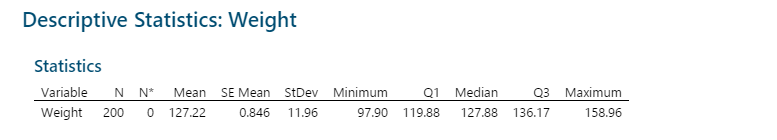
\includegraphics[width=0.9\textwidth]{q31.png}


\item Make a histogram of \textit{Weight}.  Does the data seem to have a reasonably bell-shaped distribution?  

\vspace{0.2cm}
\textit{Solution:} It looks reasonably bell-shaped.

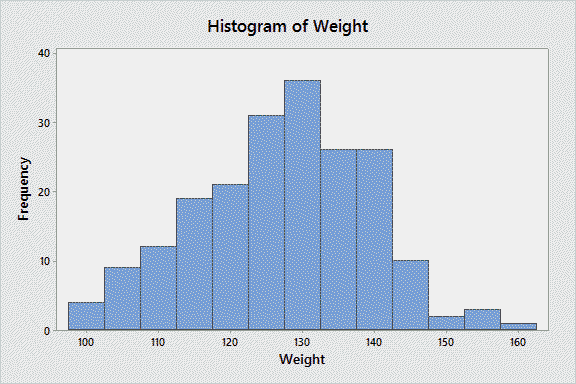
\includegraphics[width=0.8\textwidth]{q32.png}
\item Make a boxplot of \textit{Weight}.  Do you see any outliers?

\vspace{0.2cm}
\textit{Solution:} There is no outliers according to the boxplot.

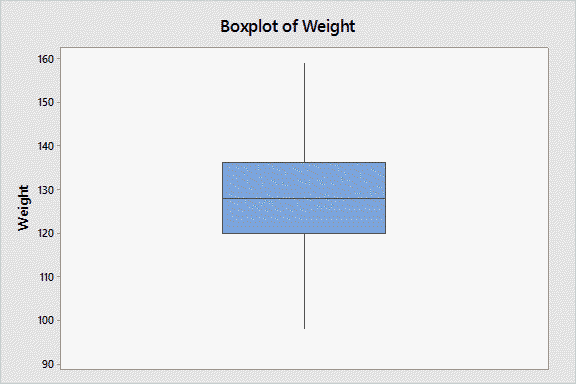
\includegraphics[width=0.8\textwidth]{q33.png}

\item Use empirical rules to complete the statements:
\begin{itemize}
\item For approximately 68\% individuals, the weight is between $[?, ?]$ 
\item For approximately 95\% individuals, the weight is between $[?, ?]$ 
\item For approximately 99.7\% individuals, the weight is between $[?, ?]$ 
\end{itemize}

\vspace{0.2cm}
\textit{Solution:} 

\begin{itemize}
\item For approximately 68\% individuals, the weight is between $[115.26, 139.18]$ 
\item For approximately 95\% individuals, the weight is between $[103.3, 151.14]$ 
\item For approximately 99.7\% individuals, the weight is between $[91.34, 163.1]$ 
\end{itemize}



\item (Optional) Look at the data. What are the true percentages in those intervals you just computed? Do they agree with the empirical rules (roughly)?

\vspace{0.2cm}
\textit{Solution:} The true percentages are very close to those given by the empirical rules:
\begin{itemize}
\item For  66.5\% individuals, the weight is between $[115.26, 139.18]$ 
\item For  94.5\% individuals, the weight is between $[103.3, 151.14]$ 
\item For  100\% individuals, the weight is between $[91.34, 163.1]$ 
\end{itemize}


\end{enumerate}
\end{problem}

\begin{problem}{}
A World Cup 2018 quarter-final between Sweden and England will happen on Jul 7. Suppose Sweden will score 0-3 goals with equal probability, and same for England. 
\begin{enumerate}
\item What is the sample space for this quarter-final?

\vspace{0.2cm}
\textit{Solution:} 
The sample space for this quarter-final is all the possible scores for $(\text{Sweden}:\text{England})$,
\begin{align*}
    \{ &(0:0),\  (0:1),\  (0:2),\  (0:3),\\
       &(1:0),\  (1:1),\  (1:2),\  (1:3),\\
       &(2:0),\  (2:1),\  (2:2),\  (2:3),\\
       &(3:0),\  (3:1),\  (3:2),\  (3:3) \}
\end{align*}
\item What is the probability that Sweden scores more goals than England? 

\vspace{0.2cm}
\textit{Solution:} 
There are a total of 16 sample points in sample space, each has probability $\frac{1}{16}$. The event ``Sweden scores more goals than England'' contains the following 6 sample points:
$$\{(1:0),\ (2:0),\ (3:0),\ (2:1),\ (3:1),\ (3:2)\}.$$
Thus the probability is $\frac{6}{16}=\frac{3}{8}$.


\end{enumerate}
\end{problem}

\begin{problem}{}
Suppose among all soccer fans, 12\% support  Sweden, 23\% support  England, and 4\% support both. A soccer fan is to be selected at random.
\begin{enumerate}

\item What is the probability that the soccer fan supports either  Sweden or  England (or both)?

\vspace{0.2cm}
\textit{Solution:} 
Let A=``Supports Sweden'', B=''Supports England''. Then by additive rule,
$$\pr(A \cup B)=\pr(A)+\pr(B)-\pr(A\cap B) = 0.12+0.23 - 0.04 =0.31. $$

\item What is the probability that the soccer fan supports neither team?

\vspace{0.2cm}
\textit{Solution:} 
The event ``Supports neither team'' is the complement of ``Supports either Sweden or England (or both)''. Thus by comlement rule,
    $$\pr((A \cup B)^c)=1-\pr(A\cup B) = 1-0.31=0.69.$$

\item What is the probability that the soccer fan supports  Sweden but not  England?
    
\vspace{0.2cm}
\textit{Solution:} 
Let C=``Supports Sweden but not England'', then $A = C \cup (A\cap B)$. Note that $C$ and $A\cap B$ are mutually exclusive. Therefore,
$$\pr(C) =\pr(A) -  \pr(A\cap B)= 0.12-0.04=0.08.$$

If any of these is not clear, drawing a diagram would help you.
\end{enumerate}
\end{problem}

\begin{problem}{}

Suppose the probability that a World Cup game will have more than 3 goals scored is 30\%, and the probability that the game will have more than 4 goals scored is 20\%.
For a World Cup game that has more than 3 goals scored, what is the
probability of it having more than 4 goals scored? 

\vspace{0.2cm}
\textit{Solution:} 
The question as asking about the conditional probability $\pr(\text{scores } 4_{+} \mid \text{scores } 3_+) $. By the definition of conditional probability,
\begin{align*}
    \pr(\text{scores } 4_{+} \mid \text{scores } 3_+) 
    &= \frac{\pr(\text{scores } 4_{+} \cap \text{scores } 3_{+})}{\pr(\text{scores } 3_+)} \\
    &=  \frac{\pr(\text{scores } 4_{+} )}{\pr(\text{scores } 3_+)} \\
    &= \frac{0.2}{0.3}=\frac{2}{3}
\end{align*}
\end{problem}


\end{document}




